\sujet{Photomosaic}

\begin{note}All documents allowed. No code is required, but pseudo-code might be provided.\end{note}

\section{Introduction}

\begin{figure}[htbp]
\centering
\subfloat[Original image.]{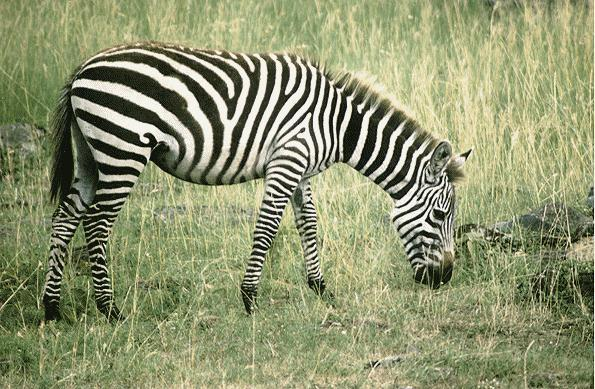
\includegraphics[width=.49\linewidth]{zebre}}
\hfill
\subfloat[Mosaic image.]{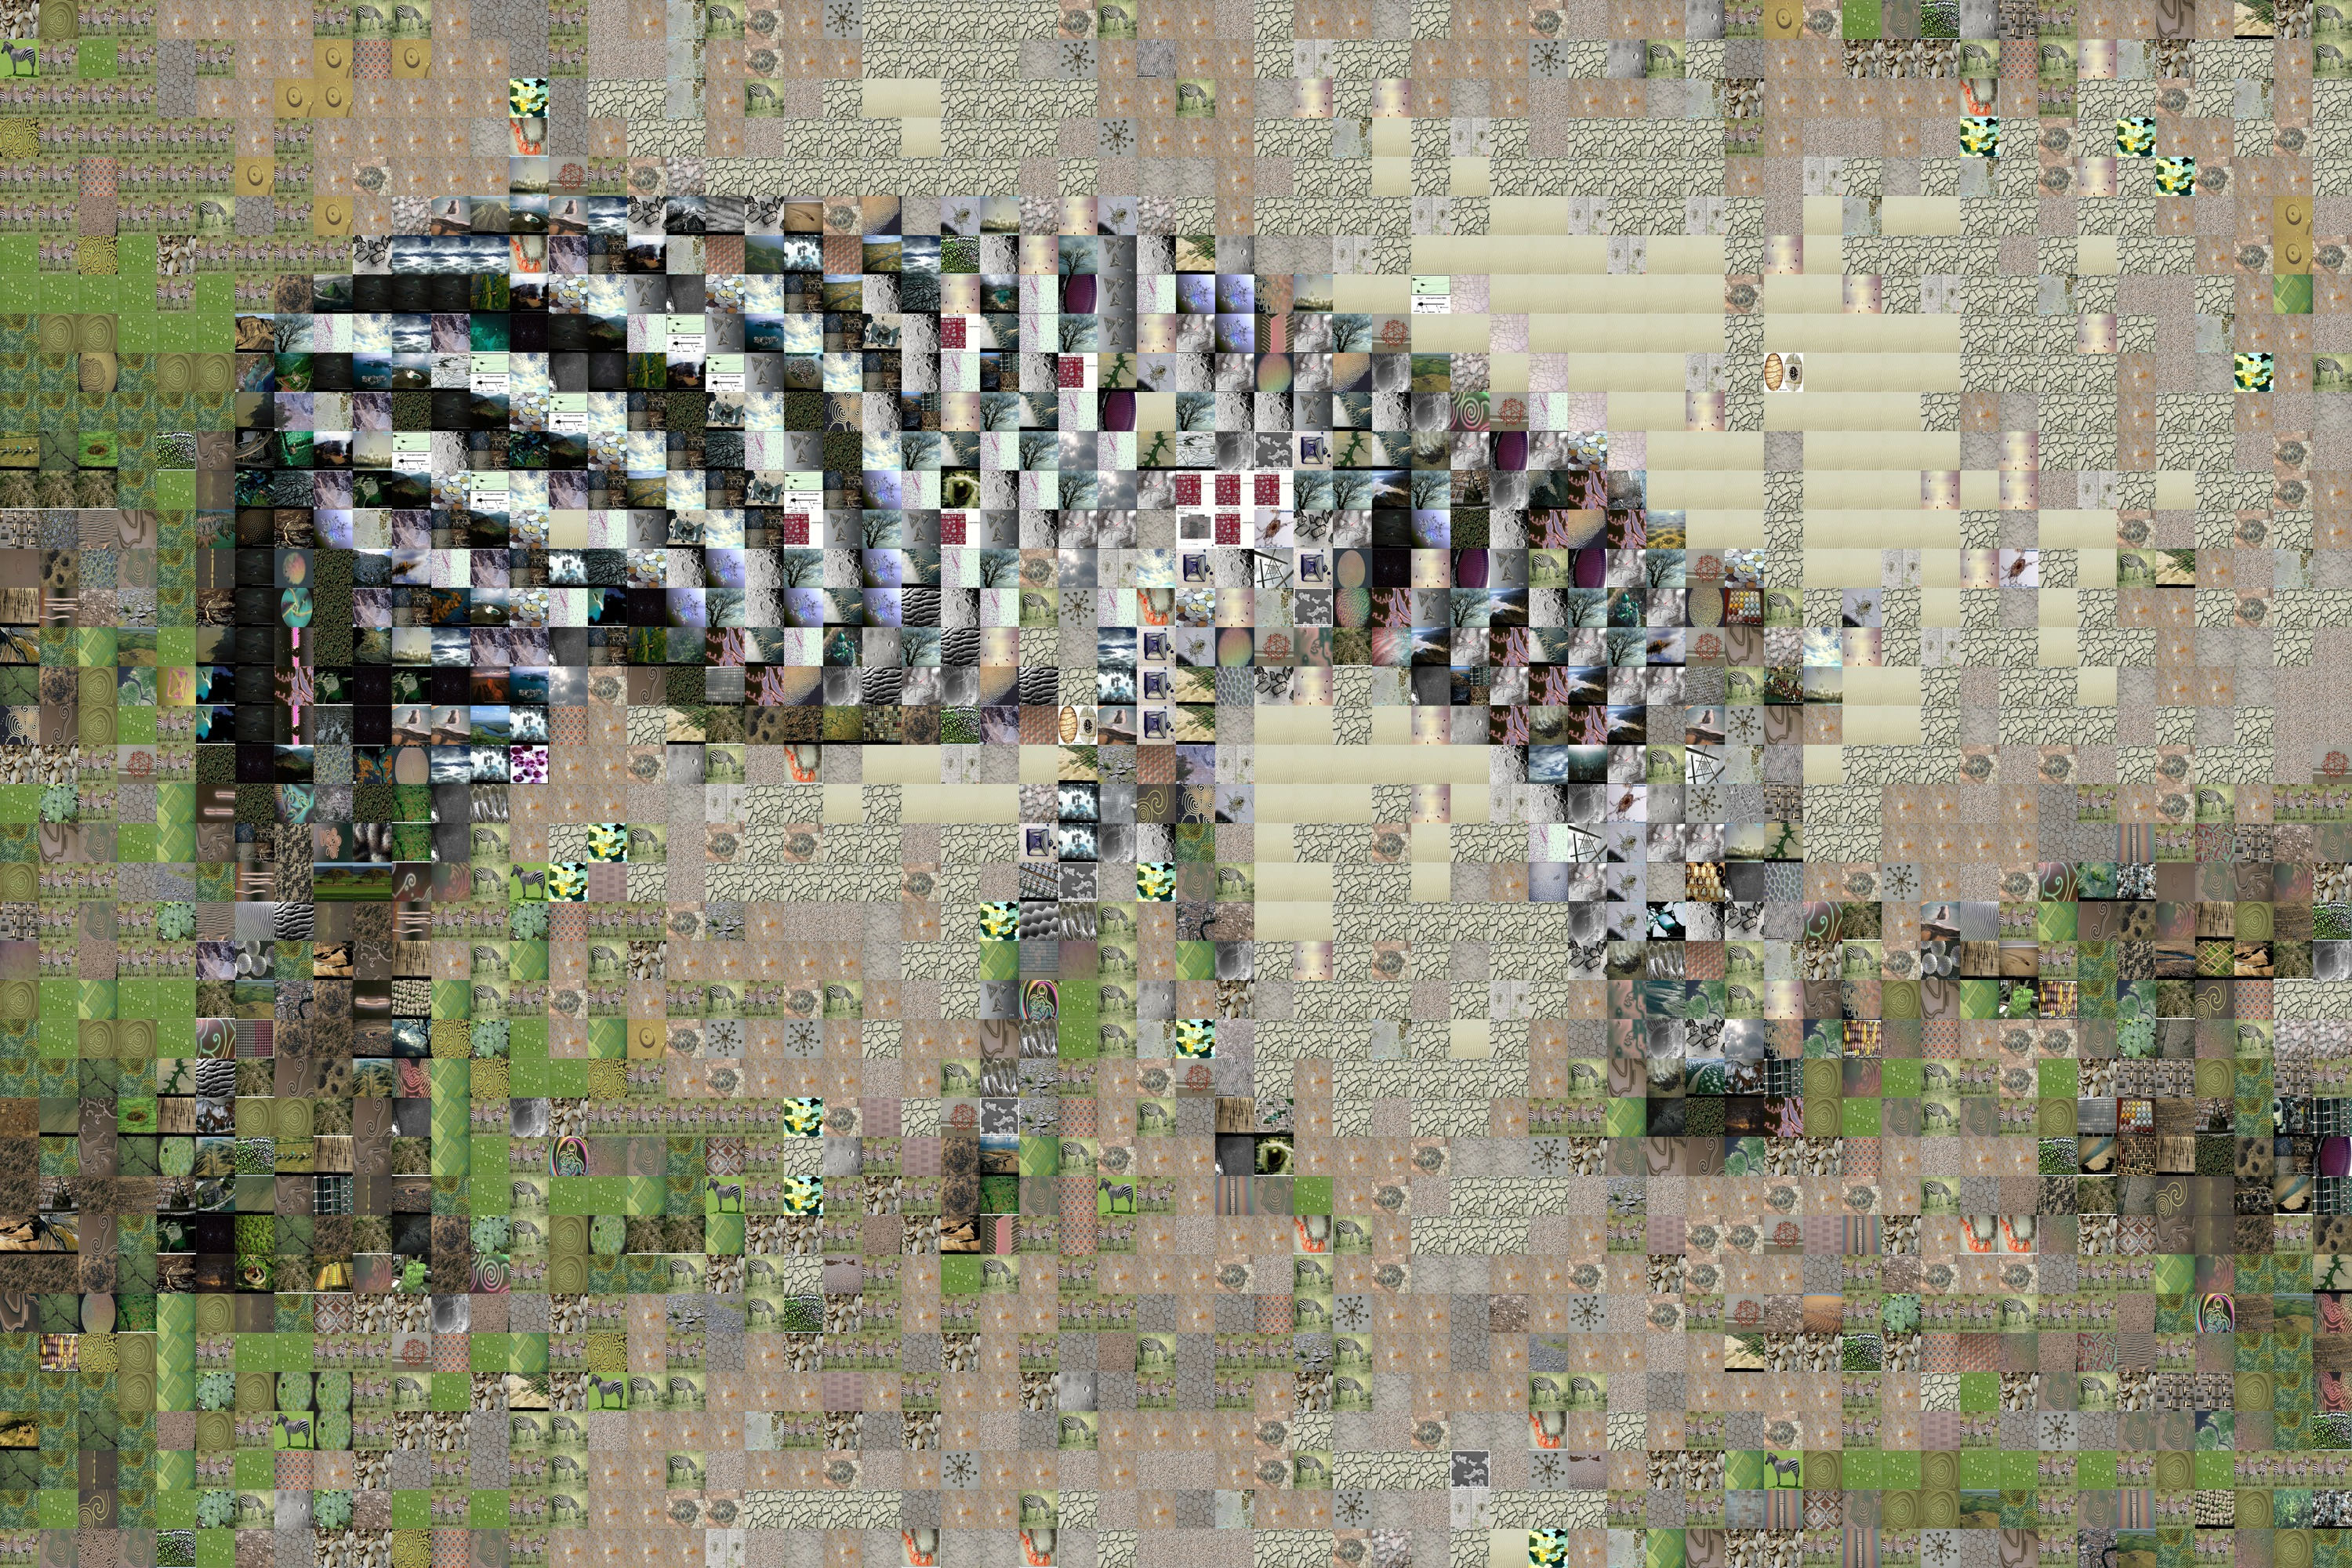
\includegraphics[width=.49\linewidth]{zebre_mosaic2.jpg}}
\caption{Mosaic example.}
\end{figure}

A photomosaic is composed of small images, stored in a database (a high number of images is required), and smartly positionned in order to correctly represent the original background image. The objective is to create a program that generates such a mosaic.

\section{Requirements (20 points)}

\begin{qbox}
Propose a method in order to construct such a mosaic. 

\begin{itemize}
 \item Detail the different steps of the algorithm. 
\item Emphasize the use of geometry in this context. 
\item Mention the computational complexity when necessary.
\end{itemize}
\end{qbox}
